\documentclass[conference]{IEEEtran}
\IEEEoverridecommandlockouts
\usepackage{cite}
\usepackage{amsmath,amssymb,amsfonts}
\usepackage{algorithmic}
\usepackage{graphicx}
\usepackage{textcomp}
\usepackage{xcolor}
\usepackage{url}
\usepackage{array}
\usepackage{tikz}
\usetikzlibrary{arrows.meta,positioning,fit,calc}
\hyphenpenalty=10000
\exhyphenpenalty=10000
\emergencystretch=1.5em
\makeatletter
\newcommand{\authorflushleft}{\end{@IEEEauthorhalign}\hskip 0pt plus -1fill\begin{@IEEEauthorhalign}}
\newcommand{\linebreakand}{\end{@IEEEauthorhalign}\par\noindent\mbox{}\begin{@IEEEauthorhalign}}
\makeatother
\def\BibTeX{{\rm B\kern-.05em{\sc i\kern-.025em b}\kern-.08em
    T\kern-.1667em\lower.7ex\hbox{E}\kern-.125emX}}

% ---------------------------------------------------------------------
\newcommand{\embmodel}{\texttt{snowflake\allowbreak-arctic\allowbreak-embed\allowbreak-xs}}
\newcommand{\embdim}{384}
\newcommand{\rerankmodel}{\texttt{ms\allowbreak-marco\allowbreak-MiniLM\allowbreak-L\allowbreak-6\allowbreak-v2}}
\newcommand{\llmname}{GPT\nobreakdash-6 Luna}
% ---------------------------------------------------------------------

\tikzset{
  box/.style={draw, rounded corners=2pt, align=center, font=\footnotesize,
              minimum height=6mm, inner sep=3pt, fill=white},
  store/.style={box, fill=gray!12},
  llm/.style={box, fill=gray!28, font=\footnotesize\bfseries},
  arr/.style={-{Stealth[length=2mm]}, semithick},
  grp/.style={draw, dashed, rounded corners=3pt, inner sep=4pt}
}

\begin{document}

\title{E.C.H.O: An Intent Aware Personal Memory System for Unified Search Across Email, Web, and Video History}

\author{\authorflushleft\IEEEauthorblockN{1\textsuperscript{st} Arjun Sai N}
\IEEEauthorblockA{\textit{Dept. of Computer Science and Engineering} \\
\textit{PES University}\\
Bengaluru, India}
\and
\IEEEauthorblockN{2\textsuperscript{nd} Mohammed Mir Fazlai Ali}
\IEEEauthorblockA{\textit{Dept. of Computer Science and Engineering} \\
\textit{PES University}\\
Bengaluru, India}
\linebreakand
\IEEEauthorblockN{3\textsuperscript{rd} Mohammed Shehzaad Khan}
\IEEEauthorblockA{\textit{Dept. of Computer Science and Engineering} \\
\textit{PES University}\\
Bengaluru, India}
\and
\IEEEauthorblockN{4\textsuperscript{th} Mrigank Jain}
\IEEEauthorblockA{\textit{Dept. of Computer Science and Engineering} \\
\textit{PES University}\\
Bengaluru, India}
\linebreakand
\IEEEauthorblockN{5\textsuperscript{th} Mannuru Shalima Sulthana}
\IEEEauthorblockA{\textit{Dept. of Computer Science and Engineering} \\
\textit{PES University}\\
Bengaluru, India}
}

\maketitle

\begin{abstract}
In a single day, a person meets information in many places, such as the inbox, the browser, and video sites. All these places keep their own history behind their own search box, so finding something again starts with guessing where it was seen. We present E.C.H.O (Efficient Contextualized History Orchestrator), a personal memory for a single user. It brings Gmail, Chrome, and YouTube activity into one store on the user's own laptop, and then it answers questions about that activity in plain language. It keeps all mail, except what Gmail itself files as spam or trash. Web pages and videos, though, get kept only if signals such as foreground time, scrolling, watch time, or a return visit show that the person actually paid attention to them. In the background, a worker cleans each item and pulls text out of its attachments. It also puts each item in one of five broad categories and embeds it for search by meaning. When a question comes in, it goes to a language model, which may call a single search tool, and this tool is plain code. It runs keyword search and vector search together, and then it fuses the two ranked lists by reciprocal rank fusion. If the results look weak, it widens the search. After that, a local cross encoder reorders what is left. A typical question costs two model calls, and the code allows at most six. Storage, indexing, and search all run locally. The model gets just the question and limited excerpts of the top results. It never sees database rows or the whole store. Apart from this, a wellbeing module describes how time is spent, and it does not judge it. It also sorts items into personal goals. It adds an item on its own only if it is confident, and the rest wait for the user to approve them. We tested all this on a collection of 119 items and 38 questions. The first ten results held 93\% of the relevant items. A question needed 2.3 model calls and a median of 8.1 seconds. And in all 13 clean scripted sessions, the capture rules agreed with their specification. The tests also show that, on this small collection, semantic search alone ranked the results better than the full pipeline. We discuss why.
\end{abstract}

\begin{IEEEkeywords}
personal information management, retrieval augmented generation, hybrid search, reciprocal rank fusion, tool calling agents, intent aware capture, local first software, digital wellbeing
\end{IEEEkeywords}

% ---------------------------------------------------------------------
\section{Introduction}
% ---------------------------------------------------------------------
Suppose a student is preparing for a job interview. The company sends an email. Over the next few days, the student reads articles about operating systems in Chrome and watches a few tutorials on YouTube. A week later, the student wants all that material back. Now the email sits in Gmail, the videos sit in the YouTube watch list, and the articles are buried in the browser history. All these apps have their own search box, and none of them knows about the other two. So the student either searches all three, one at a time, or starts again from scratch.

The idea of a machine that remembers what its owner has seen is not new. Bush called it the memex in 1945 \cite{b1}. Later systems such as Stuff I've Seen \cite{b2} and MyLifeBits \cite{b3} built personal stores of mail, pages, and documents. But two problems still make such systems hard to use every day. The first problem is noise. A browser logs every page that opens, even stray clicks and tabs closed after two seconds. So if a memory is built directly on that log, it fills up with things nobody read. The second problem is recall by exact words. A search box needs the right keyword, but people remember loosely, as in ``the OS material I read after the interview email.''

E.C.H.O handles both problems. It watches Gmail, Chrome, and YouTube, but it keeps a page or a video only if engagement shows real attention. All items share one data model on the user's laptop. There they are enriched in the background, and the user can ask about them in natural language. Every answer is grounded in the stored items, and this follows retrieval augmented generation \cite{b4}.

The main contributions are:
\begin{itemize}
\item An intent aware capture layer, with a separate rule set for each source and privacy filters that act before anything is stored. Here, sensitive pages lose their text, secret parameters are cut from addresses, and private work apps give just a page title.
\item A local storage model where emails, pages, and videos share one central table. PostgreSQL is the permanent record, Redis holds short lived state, and the FAISS index can be rebuilt from PostgreSQL. E.C.H.O also extracts attachment text when the mail arrives, so it is searchable as well.
\item A bounded agentic retrieval loop. The language model plans and phrases the searches, and a deterministic tool does the actual searching. This tool runs hybrid keyword and vector search, rank fusion, a rule based quality check with widening, and cross encoder reranking. A typical question needs two model calls, and the code sets a hard limit of six.
\item A wellbeing module that reports time, sessions, and self declared regret only in descriptive terms. Along with it comes a grouping engine for personal goals. This engine files an item on its own only when two signals agree, and the user can undo that in one click. Every other item waits for the user to approve it.
\end{itemize}

Section~\ref{sec:related} reviews related work, and Section~\ref{sec:overview} gives an overview of the system. Next, Section~\ref{sec:method} covers capture, storage, enrichment, and retrieval, and Section~\ref{sec:wba} describes the wellbeing module and the user groups. Section~\ref{sec:privacy} then covers privacy, and Section~\ref{sec:impl} covers the implementation. Section~\ref{sec:eval} has the evaluation. Finally, Section~\ref{sec:limits} lists the limitations, and Section~\ref{sec:conc} concludes.

% ---------------------------------------------------------------------
\section{Related Work}\label{sec:related}
% ---------------------------------------------------------------------
\subsection{Personal Information Management}
Bush imagined the memex as a desk that holds a person's books, records, and letters and brings any of them back quickly \cite{b1}. Stuff I've Seen built one index over everything a person had already seen, such as an email, a web page, or a document. It used that earlier exposure as a cue for search \cite{b2}. MyLifeBits kept personal data in a SQL database, and its aim was to store everything that could be captured \cite{b3}. E.C.H.O has the same goal of refinding, but it differs in two ways. First, it filters at capture time, so it does not store everything. Second, it goes a step beyond a query box and answers questions in natural language.

\subsection{Retrieval Augmented Generation and Tool Use}
Retrieval augmented generation couples a retriever with a text generator, so that the generated answer draws on the retrieved documents \cite{b4}. E.C.H.O applies this idea to a personal collection and arranges the steps as a graph built with LangGraph \cite{b5}. ReAct showed that a language model can alternate between reasoning and actions such as search calls, and that grounding each step in tool output reduces invented facts \cite{b13}. We borrow this pattern, but in a deliberately narrow form. The model has exactly one read only tool. Apart from two small local encoders, this tool has no model inside it. Also, the code caps how many rounds the model gets.

\subsection{Hybrid Search and Reranking}
Sentence embeddings such as Sentence BERT let us compare texts by meaning, using cosine similarity \cite{b6}. E.C.H.O embeds every item with a small local sentence model \cite{b16} and searches the vectors with FAISS \cite{b8}. For keyword search, it uses the full text search built into PostgreSQL. The problem is that these two methods score on unrelated scales, so it does not make sense to add their scores directly. Reciprocal rank fusion solves this because it uses just the position of each item in each list \cite{b9}. After fusion, a cross encoder reads the question and a candidate together and scores how well they match. Nogueira and Cho showed that this works well for passage reranking \cite{b10}. Our cross encoder is a compact MiniLM \cite{b7} model, trained on the MS MARCO passage ranking data \cite{b11}.

\subsection{Local First Software}
Kleppmann et al.\ describe local first software, where users own their data and the application works from a copy on their own device \cite{b12}. E.C.H.O follows the same idea, as the database, the vector index, the cache, and both encoders all run on the user's laptop. The hosted language model gets only limited pieces of text.

\subsection{Digital Wellbeing Tools}
Lyngs et al.\ reviewed hundreds of digital self control apps and browser extensions. They found that most of them block, limit, or track usage against a goal \cite{b14}. E.C.H.O is different from these tools. It just shows where the time went and lets the user mark the items they regret. It does not score the user or block any content. It also does not call any time wasted.

% ---------------------------------------------------------------------
\section{System Overview}\label{sec:overview}
% ---------------------------------------------------------------------
Fig.~\ref{fig:arch} shows the main parts of the system. First, data comes in through three connectors. The Gmail connector reads mail through the Gmail API with OAuth, and it asks only for the changes since its last check. A Chrome extension watches desktop browsing and YouTube playback, and the YouTube connector then fills in the video details from the YouTube Data API. All connectors hand their items to one FastAPI gateway. There, the storage engine writes each item in a single transaction and skips duplicates.

Next, there are three stores, and each one has a separate job. PostgreSQL is the permanent record of every item. FAISS holds the embedding vectors, and it can be rebuilt from PostgreSQL. Redis keeps the short lived state, which covers revisit flags, cached attachment text, reminder state, and the user's capture settings. This entire storage layer runs on the user's laptop.

Three modules then work on the stored data. The enrichment worker prepares new items for search in the background, and the retrieval engine answers the questions. The wellbeing module turns the stored activity into time summaries, sessions, regret patterns, and group suggestions. The main interface is a React dashboard, and a small extension popup lets the user pause capture.

\begin{figure}[t]
\centering
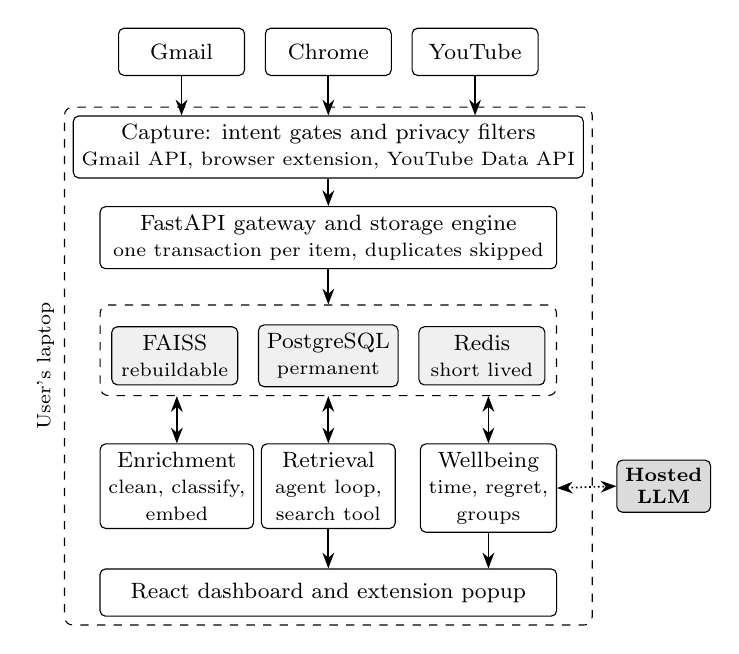
\begin{tikzpicture}[node distance=3.5mm and 2.5mm]
  \node[box, minimum width=16mm] (gm) {Gmail};
  \node[box, minimum width=16mm, right=of gm] (ch) {Chrome};
  \node[box, minimum width=16mm, right=of ch] (yt) {YouTube};
  \node[box, minimum width=58mm, below=5mm of ch] (cap)
      {Capture: intent gates and privacy filters\\ \scriptsize Gmail API, browser extension, YouTube Data API};
  \node[box, minimum width=58mm, below=of cap] (gw)
      {FastAPI gateway and storage engine\\ \scriptsize one transaction per item, duplicates skipped};
  \node[store, minimum width=16mm, below=7mm of gw] (pg) {PostgreSQL\\ \scriptsize permanent};
  \node[store, minimum width=16mm, left=of pg] (fa) {FAISS\\ \scriptsize rebuildable};
  \node[store, minimum width=16mm, right=of pg] (rd) {Redis\\ \scriptsize short lived};
  \node[grp, fit=(fa)(pg)(rd), inner ysep=5pt, yshift=2pt] (st) {};
  \node[box, minimum width=17mm, below=6mm of st.south west, anchor=north west] (enp)
      {Enrichment\\ \scriptsize clean, classify,\\ \scriptsize embed};
  \node[box, minimum width=17mm, below=6mm of st.south, anchor=north] (rse)
      {Retrieval\\ \scriptsize agent loop,\\ \scriptsize search tool};
  \node[box, minimum width=17mm, below=6mm of st.south east, anchor=north east] (wba)
      {Wellbeing\\ \scriptsize time, regret,\\ \scriptsize groups};
  \node[box, minimum width=58mm, below=5mm of rse] (ui) {React dashboard and extension popup};
  \node[grp, fit=(cap)(gw)(st)(enp)(wba)(ui), inner sep=3pt] (lap) {};
  \node[font=\scriptsize, rotate=90, anchor=south] at (lap.west) {User's laptop};
  \node[llm, minimum width=11mm, right=3mm of lap.east |- rse.east, anchor=west, font=\scriptsize\bfseries] (lm) {Hosted\\LLM};
  \draw[arr] (gm) -- (gm |- cap.north);
  \draw[arr] (ch) -- (cap);
  \draw[arr] (yt) -- (yt |- cap.north);
  \draw[arr] (cap) -- (gw);
  \draw[arr] (gw) -- (st.north);
  \draw[arr, {Stealth[length=2mm]}-{Stealth[length=2mm]}] (enp.north) -- (enp.north |- st.south);
  \draw[arr, {Stealth[length=2mm]}-{Stealth[length=2mm]}] (rse.north) -- (rse.north |- st.south);
  \draw[arr, {Stealth[length=2mm]}-{Stealth[length=2mm]}] (wba.north) -- (wba.north |- st.south);
  \draw[arr] (rse) -- (ui);
  \draw[arr] (wba.south) -- (wba.south |- ui.north);
  \draw[arr, densely dotted, {Stealth[length=2mm]}-{Stealth[length=2mm]}] (wba.east) -- (lm.west);
\end{tikzpicture}
\caption{Main parts of E.C.H.O. Everything inside the dashed frame runs on the user's laptop. The dotted arrow is the only path to the hosted language model of E.C.H.O; it carries bounded text from three callers (classification, retrieval, weekly reflection), described in Section~\ref{sec:privacy}.}
\label{fig:arch}
\end{figure}

% ---------------------------------------------------------------------
\section{Methodology}\label{sec:method}
% ---------------------------------------------------------------------
\subsection{Intent Aware Capture}
What should E.C.H.O keep? Each source has its own answer, and Table~\ref{tab:gates} summarizes them. These are the values we chose for the final system. The browser and the server hold matching copies, so that the server does not silently refuse a page that the extension sends.

Gmail is treated differently from the other two sources. Mail arrives on its own, so the user does not choose it. Also, few mails arrive each day, and even an unread message may matter later. So we store all messages when they arrive. The connector polls every 30 seconds, but each poll asks Gmail just for the changes since a saved history position. It does not list the entire mailbox each time. If that position has expired, the connector will list the mailbox once. Then the uniqueness rule on stored items absorbs the overlap. We do not read mail that Gmail has already filed as spam or trash, so Gmail's own spam filter also works as the spam filter of E.C.H.O. Whenever the user opens a message in Gmail on the web, the extension reports just the message id and the seconds spent reading.

A Chrome page has to pass a two phase gate. In phase one, the page has to stay in the foreground for at least five seconds. If a page fails this phase, we drop it, and we remember only a page that passes it for revisit detection. Phase two comes next, where at least one sign of attention has to appear. This sign can be enough foreground time, enough scrolling, a real interaction, or a visit to the same page within the last 24 hours. Selecting text or clicking inside the page counts as an interaction, but clicking a link does not. This is because a click that leaves the page shows a choice to go elsewhere, and not interest in the page itself. We count time only while the tab is active, the window has focus, and the user has not been idle for 30 seconds. Along with the text of the main content, the extension also sends the top level headings of the page, so that the page can be found later by its topic.

We keep a YouTube video if the user watches it long enough, or watches a large enough share of it. Pausing, seeking, changing the speed, or returning to the same video within a day also keeps it. The completion rule needs at least five seconds of real watching, such that swiping past a short clip does not count as watching ten percent of it. Once a video has been watched for five seconds, the extension records the visit, so that a second short visit can pass through the revisit rule. We recognize Shorts from the page address itself, and they have a lower time bar.

\begin{table}[t]
\caption{Capture Rules for Each Source}
\label{tab:gates}
\centering
\renewcommand{\arraystretch}{1.15}
\begin{tabular}{|>{\raggedright\arraybackslash}p{1.35cm}|>{\raggedright\arraybackslash}p{6.2cm}|}
\hline
\textbf{Source} & \textbf{An item is kept when} \\
\hline
Gmail & Always, at arrival, except mail in Spam or Trash. Polled every 30~s for changes only. Reading time is added when a message is opened (opens under 3~s are ignored). \\
\hline
Chrome & Phase 1: at least 5~s in the foreground. Phase 2: any one of at least 10~s in the foreground, at least 15\% scroll depth, one interaction other than a link click, or a revisit within 24~hours. Work app pages: at least 5~s or one interaction, title only. \\
\hline
YouTube & Any one of at least 20~s of foreground playback (10~s for Shorts), at least 10\% of the video watched with at least 5~s of watching, a pause, seek, or speed change by the user, or a revisit within 24~hours. \\
\hline
\end{tabular}
\end{table}

\subsection{Storage Model}
How does an item look in storage? Each email, page, and video becomes one row in a central table of memory items. Fields that belong to a particular source go into a matching table for Gmail, Chrome, or YouTube, and attachments get a table of their own. Engagement counters such as reading time, watch time, and revisits change often, so we keep them separately. Also, Chrome and YouTube write one row for every admitted visit, with the visit time and the seconds spent. This way, a page read on two different days counts on both days. The complete schema has 17 tables.

A uniqueness rule on the pair of source type and source id stops the same item from being stored twice, for example after a connector restarts. All items always carry one of the five system groups, and misc is the fallback. We first write an item in a raw state and flag it as unprocessed. This keeps the capture path short and safe against crashes. Later, if a revisited page comes back with different text, we flag it again, so that its vector will be rebuilt. We store timestamps in UTC and show them to the user in local time.

A user can delete a single item, and that hides it from all queries. Apart from this, a retention setting lets the user keep items forever, for one year, or for six months. Recalling old things is the whole point of the system. This is why keeping items forever is the default. If the user picks a shorter window, a job at backend startup will permanently remove the older items from PostgreSQL, the FAISS index, and Redis together.

\subsection{Background Enrichment}
A background worker picks up the unprocessed items every few seconds. It runs outside the capture path, so a slow enrichment step can never slow down capture. Each item then goes through four steps.

\textit{Cleaning.} For email, HTML is converted to text with the line breaks kept, and scripts, styles, tracking pixels, and hidden preview text are removed. When the sending app has split a body around an inline image, the parts are joined back together. Quoted earlier messages are removed, but the lines the sender typed between quoted lines are kept. This is because an inline reply is often the most important part of the message. A heuristic remover that we tested cut real body text in six of eight sample messages, while a leftover signature only adds a little noise. So signatures are deliberately left in place, as a little noise is better than lost body text. For a reply, keywords from earlier messages in the same thread are added, so that a terse ``Re:'' can still be found by its topic. For web pages, the extension has already picked the main content and the headings, and the worker separates the headings from the body. A video's text is made of its title, channel, category, tags, and description. The server also tries to download the caption text, but this is best effort, and it returned nothing for any of the 14 videos in our test data.

\textit{Attachments.} The same worker extracts attachment text when the mail is processed. It supports PDF, DOCX, XLSX, PPTX, HTML, forwarded messages, and plain text formats such as TXT, CSV, Markdown, JSON, and calendar files. Images and scanned PDFs are read with Tesseract OCR \cite{b15}, while inline images such as signature logos, and very small images, are skipped. The extracted text is stored next to the attachment record and not inside the email body. The beginning of each attachment joins the embedded text of the email, while the entire text joins the keyword index. So content deep inside a file can still be found by keyword.

\textit{Embedding.} The cleaned text is turned into a \embdim{} dimension vector with the \embmodel{} sentence model \cite{b16}, which reads up to 512 tokens. The text is assembled such that the short hints come first. They are the subject, keywords, and sender for mail, the domain and headings for pages, and the channel and category for videos. Long text such as a body or a description comes last. Then the text is cut to the 512 token window of the model, using the model's own tokenizer and ending at a whole word. So only the end of the long part is removed, and the stored text is exactly what was embedded. For mail with attachments, the body takes up to 300 tokens and the attachments fill the rest. For a video, the description takes up to 200 tokens and any caption text fills the rest. The vector is then added to the FAISS index without a rebuild.

\textit{Classification.} Every item receives one of five broad groups, which are work, study, entertainment, personal, and misc. The group is chosen by a four stage cascade. Stage one reads structural signals from the source, such as Gmail category labels, academic mail domains, or the YouTube video category. Next, stage two looks up the web domain in a curated table. Then stage three compares the vector of the item with a center point for each group and accepts only a clear winner. Each center starts as the mean of several example sentences written for its group. While a center is still a seed, the required lead is smaller, 0.05 instead of 0.08, as we measured on labeled rows (Section~\ref{sec:eval}). Once a group has at least ten confirmed items, its center is recomputed from real items. Each source is weighted equally here, so that a center learns a topic and not the look of one particular source. Both kinds of center need a cosine similarity of at least 0.55. A recomputed center must also lead the second best group by at least 0.08. The recomputation runs when the worker starts, if the stored centers are missing or older than 30 days. Finally, stage four asks the language model, one item at a time, using only the title and about 300 characters of text. With an OpenAI model, the call is a typed choice among the five group names. With other providers, the reply must be exactly one group name, and any other reply becomes misc. If the typed call raises an error, that item takes the single word path instead, so classification does not stop. No confidence value is stored.

\textit{State tracking.} Each item ends as either processed or failed. Failed items are kept apart, so a failure is not counted as done, and it is not lost either. A configuration switch lets the worker try them again.

\subsection{Retrieval Loop}
How is a question answered? It goes through the loop in Fig.~\ref{fig:graph}. The language model, \llmname{}, gets the conversation so far, a small calendar around today's date, the question, and one tool called \texttt{search\_memories}. The tool takes a query of a few keywords. It also takes some options. These are up to two alternative phrasings, a list of sources, a start date, a reference item with the word before or after, and a flag to ask for attachment text. The model decides how to phrase the search. Then, in one round, it may issue several searches in parallel, for instance one per source. After reading the results, it either answers directly or searches again. On the first turn of a chat, the first call has to use the tool. A usual question needs one call that searches and one call that answers. The code allows at most five searches for one question, and at most three in one round. After the fifth search, we make the next call without the tool, such that the model has to answer. So a question costs between two and six model calls, and the program enforces this bound, not the prompt.

\begin{figure}[t]
\centering
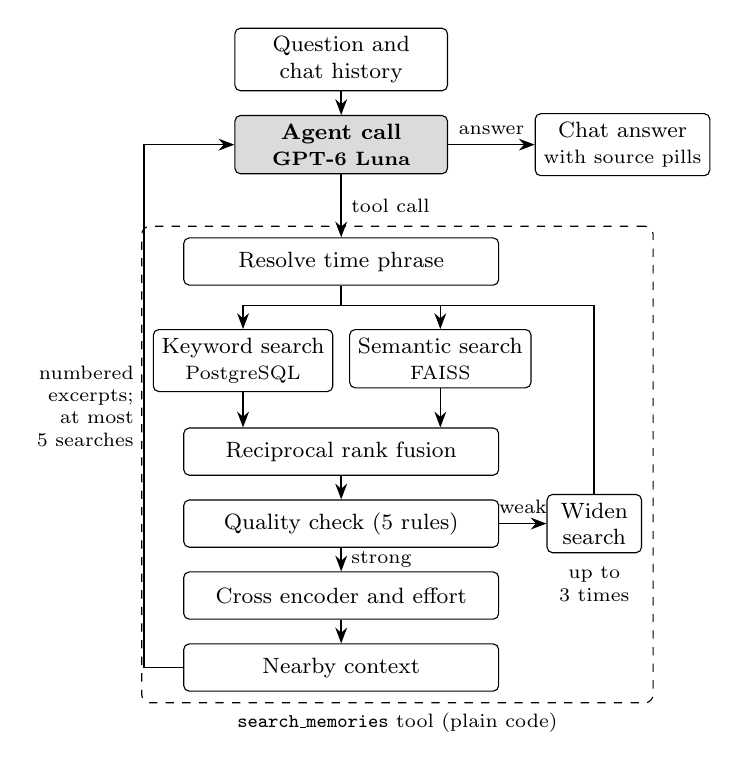
\begin{tikzpicture}[node distance=3mm and 3mm]
  \node[box, minimum width=27mm] (q) {Question and\\ chat history};
  \node[llm, minimum width=27mm, below=of q] (ag) {Agent call\\ \scriptsize\llmname};
  \node[box, minimum width=22mm, right=11mm of ag] (an) {Chat answer\\ \scriptsize with source pills};
  \node[box, minimum width=40mm, below=8mm of ag] (ta) {Resolve time phrase};
  \coordinate (bus) at ($(ta.south)+(0,-2.5mm)$);
  \node[box, minimum width=19mm, anchor=north east] (kw) at ($(bus)+(-1mm,-3mm)$) {Keyword search\\ \scriptsize PostgreSQL};
  \node[box, minimum width=19mm, anchor=north west] (se) at ($(bus)+(1mm,-3mm)$) {Semantic search\\ \scriptsize FAISS};
  \node[box, minimum width=40mm, anchor=north] (rrf) at ($(bus)+(0,-15.5mm)$) {Reciprocal rank fusion};
  \node[box, minimum width=40mm, below=of rrf] (qc) {Quality check (5 rules)};
  \node[box, minimum width=12mm, right=6mm of qc] (wd) {Widen\\search};
  \node[box, minimum width=40mm, below=of qc] (ce) {Cross encoder and effort};
  \node[box, minimum width=40mm, below=of ce] (nb) {Nearby context};
  \node[grp, fit=(ta)(kw)(se)(rrf)(qc)(wd)(ce)(nb), inner sep=4pt] (tool) {};
  \node[font=\scriptsize, anchor=north] at (tool.south) {\texttt{search\_memories} tool (plain code)};
  \draw[arr] (q) -- (ag);
  \draw[arr] (ag) -- node[above, font=\scriptsize] {answer} (an);
  \draw[arr] (ag) -- node[right, font=\scriptsize] {tool call} (ta);
  \draw[semithick] (ta.south) -- (bus);
  \draw[semithick] (bus -| kw.center) -- (bus -| wd.center);
  \draw[arr] (bus -| kw.center) -- (kw.north);
  \draw[arr] (bus -| se.center) -- (se.north);
  \draw[semithick] (wd.north) -- (wd.north |- bus);
  \node[font=\scriptsize, align=center, below=0.5mm of wd] {up to\\3 times};
  \draw[arr] (kw.south) -- (kw.south |- rrf.north);
  \draw[arr] (se.south) -- (se.south |- rrf.north);
  \draw[arr] (rrf) -- (qc);
  \draw[arr] (qc) -- node[above, font=\scriptsize] {weak} (wd);
  \draw[arr] (qc) -- node[right, font=\scriptsize] {strong} (ce);
  \draw[arr] (ce) -- (nb);
  \draw[arr] (nb.west) -- ++(-5mm,0) |- node[pos=0.25, left, font=\scriptsize, align=right] {numbered\\excerpts;\\at most\\5 searches} (ag.west);
\end{tikzpicture}
\caption{The retrieval loop. The shaded box is the only place a language model is called. Everything inside the dashed frame is deterministic code with two small local encoders. When the search is widened, both search branches run again.}
\label{fig:graph}
\end{figure}

\textit{Resolve time phrase.} The model reads the calendar in its first message and passes a start date, so a phrase such as ``last Tuesday'' reaches the tool as a date. The tool accepts only a valid date. A phrase that points at another item, such as ``after the interview email,'' is passed as a reference item, and the code looks it up among the user's own items. This lookup goes first by keyword and then by meaning, with a minimum similarity. The time of the matching item then becomes a hard limit for both search branches. If no reference item is found, the search runs without that limit. Mail is matched by when it arrived, while pages and videos match when any of their recorded visits falls in the range. The date filter is open ended, so the answering call is told today's date and asked to use only the items inside the period the user named.

\textit{Parallel search.} The keyword branch runs the PostgreSQL full text search over a stored text index. This index covers titles, the complete item text, attachment text, senders, domains, and channel names. The semantic branch embeds the query and searches FAISS. Both branches run in the same step of the graph.

\textit{Fusion.} The two ranked lists are merged with reciprocal rank fusion \cite{b9}. For an item $d$, the fused score is
\begin{equation}
\mathrm{RRF}(d) = \sum_{b \in B} \frac{1}{k + r_b(d)}, \label{eq:rrf}
\end{equation}
where $B$ is the set of branches that returned $d$, $r_b(d)$ is its position in branch $b$ starting from 1, and $k = 60$. Since only the positions count, the two score scales do not have to be matched at all. The top 50 fused items move on to the next step.

\textit{Quality check and widening.} Five rules judge the fused list. The list is weak or empty when it has no items or holds fewer than two items. It is also weak when no item comes from a source the user asked for, or when no item falls inside the time window. The last rule checks the best cosine similarity, and a list whose best value is below 0.55 is weak as well. On our test questions, this floor flagged none of the 38 answerable queries as weak and let 2 of 12 unanswerable queries pass (Section~\ref{sec:eval}). A weak list triggers a wider search, and both branches run again. Each attempt relaxes the search more than the one before. The first attempt stretches the time window by four days, opens all sources, or shortens the query to its core keyword. The second then drops the time filter and the anchor, and the third drops the keyword filters and searches a larger part of the vector index. After three attempts, the tool reports that nothing was found, and the model can either say so or try a different phrasing.

\textit{Reranking.} The local cross encoder \rerankmodel{} \cite{b10}, \cite{b11} scores each remaining item against the question. It reads the title of the item followed by the beginning of its cleaned text, 512 characters in all. The final score blends this with an effort score:
\begin{equation}
s(d) = 0.8\,\sigma\big(c(q,d)\big) + 0.2\,e(d), \label{eq:final}
\end{equation}
where $c(q,d)$ is the cross encoder output for question $q$ and item $d$, $\sigma$ is the sigmoid function, and $e(d) \in [0,1]$ is the effort score. Effort is the mean of the engagement signals that an item has, such as reading or watch time, scroll depth, revisits, interactions, and how much of a video was watched. Each signal is capped and scaled to $[0,1]$. This favors the items that the user gave real attention to. Email is a special case. If a mail was read on a phone, or never opened in the browser, it has no measurable reading time. Instead of scoring such mail as zero, the reranker gives it the median effort of the other emails in the same result list. This way, an unmeasured email is neither punished nor promoted. By design, the score has no term for how recent an item is, and there is no diversity reranking.

\textit{Nearby context and excerpts.} For the top three items, the tool also adds their close neighbors. These are other emails in the same thread, or pages and videos from the same browsing session or within five minutes. Each result reaches the model as a numbered entry. This entry holds its title, source, time, the sender, site, or channel, and the beginning of its cleaned text. That excerpt is at most 8,000 characters for each of the top three results and 2,000 characters for the others. Suppose the question is about the content of a file attached to an email. Then the tool adds the extracted text of the attachment of the best ranked mail, up to 40,000 characters. The numbers stay the same across the searches of one question, so that a citation always points to the exact same item.

\textit{Writing the answer.} The final call writes a conversational reply in Markdown. This reply starts with the direct answer and admits gaps plainly, and when the question is ambiguous, it asks back in one line. After each fact, the reply places a hidden marker that names the numbered item supporting it. The backend keeps only the markers that point to items the tool actually returned, so that the model cannot cite a source it did not see. The dashboard then turns each marker into a small pill. This pill names the human anchor of the memory, such as the sender, the site, or the channel, along with a short date. Clicking the pill opens the original email, page, or video. Also, a thin time strip under the reply places each cited item on a timeline. While the loop runs, the dashboard shows progress messages, such as which source is being searched, and then it shows the reply.

\textit{Failure handling.} If the model cannot be reached, the deterministic pipeline runs once on the raw question. In this case, the user still receives the ranked list of matching items, and not an error.

\subsection{Conversation Memory}
Each chat has a session id, and we save every turn in PostgreSQL on the laptop. When the user opens an old chat, its session picks up from where it was left. So a follow up such as ``show me Chrome pages about that topic after that email'' can refer back to an earlier answer. At each turn, the model gets the last twelve messages of the chat, with each question cut to 1,000 characters and each answer to 3,000. The citation numbers restart with every question. At startup, we remove chat history older than 30 days.

% ---------------------------------------------------------------------
\section{Wellbeing and User Groups}\label{sec:wba}
% ---------------------------------------------------------------------
The wellbeing module answers one question: where did my time go? It describes how time is spent, but it does not judge it. So it just shows the numbers and patterns, and it leaves the verdict to the user.

\textit{Time.} Time totals are computed on demand from the stored records and are not stored separately. This avoids counting the same minutes twice. Page and video time come from the per visit rows, so each day receives exactly the time spent on that particular day. Email time comes from the reading time that the extension reports. All days are the local days of the user.

\textit{Sessions.} A session is a run of activity in which consecutive items are less than 20 minutes apart. A shorter gap would split one sitting in two. Suppose the user reads a page for 15 minutes and then opens the next page. As each item is recorded at one point in time, that read looks like a 15 minute gap. For each session, the module records its length, the system group with the most time, and how often the user switched between sources.

\textit{Regret.} It is the user who decides what is regrettable, and any item can be marked. Every mark or unmark is stored as a new event, so the record is not overwritten. An item is currently regretted when its count of events is odd. The module then reports how many marked items fall in each content type and hour. It also flags a habit when the same kind of item, at a similar hour, is marked at least three times in 30 days.

\textit{Weekly reflection.} Once a week, the module can write a short reflection. For this, one language model call receives only aggregated numbers, which are totals per category, regret counts, session patterns, and peak hours. It does not receive a title, an address, or any text from an item. Before the reply is shown, it is checked for judging phrases. If it fails this check, or if the call itself fails, a simple summary built from the same numbers is shown instead.

\textit{User groups.} System groups answer ``what kind of item is this?'', while user groups answer ``which of my goals does it serve?'', for example ``Placement prep.'' A user group starts with the items that the user files by hand. Once it has five confirmed items, an assignment job scores other items against it in two ways. The first way uses the rules the user wrote, each on a keyword, domain, channel, sender, or date range. The second way is a nearest neighbor score, which is the mean cosine similarity between the item and the three most similar confirmed members. An item is suggested when a rule matches, or when the neighbor score alone reaches a threshold. We set this threshold to 0.85, the lowest value at which no item outside a group scored at or above it in our test (Section~\ref{sec:eval}). The module can also propose a new rule when at least five confirmed members share a domain, sender, or channel.

When does E.C.H.O add something on its own? It does so only for a confident suggestion. A suggestion is confident if a rule matches and the neighbor score also reaches that same threshold. We add such an item directly, but the item still appears in the weekly review, where one click undoes it. So we handle confident items with a human on the loop. Anything less certain waits for an explicit accept in the review screen, which means the human stays in the loop. Also, an automatic addition does not count as a confirmed member until the user keeps it. So one wrong addition cannot pull in the next similar item. Manual filing and automatic additions pass through the same recorded path, so each membership has an audit trail. We never offer a rejected or removed suggestion again for that group. User groups are independent of the five system groups and have no parent among them, such that one goal can hold study pages and work mail together.

% ---------------------------------------------------------------------
\section{Privacy by Design}\label{sec:privacy}
% ---------------------------------------------------------------------
\textit{What is never captured.} Nothing from incognito windows is recorded, and the same goes for typed text and form input. Some pages also keep no text at all. A page falls in this case when its address contains a sensitive word, such as login, password, checkout, otp, or netbanking. Each word is matched as a whole word against a fixed list of 38. A page with a visible password box, or with a form of several personal fields, is treated the same way. Parameters that often carry secrets, such as tokens, one time codes, and session ids, are cut from every address before it is stored. Seven work apps, which are Slack, Atlassian, Notion, Figma, Linear, Trello, and Asana, are stored only as page titles and not as text. Their public help, blog, and documentation sections are still treated as ordinary pages. Gmail on the web is skipped by browser capture, because the mail already arrives through the Gmail API. All these lists live in one copy on the server, and the extension fetches them at startup. Until they arrive, the extension extracts no text.

\textit{What leaves the laptop.} The database, the vector index, the cache, and both encoders run locally. Two kinds of traffic leave the machine. First, requests to the Gmail and YouTube APIs fetch the user's own data. Second, calls to the hosted language model carry text from three callers. Retrieval sends the question, the recent chat history, and the numbered results. Each result is a title, a time, a sender, site, or channel, and the beginning of its text, at most 8,000 characters for each of the top three results and 2,000 for the others. When the user asks about a file, the text of one attachment is added, at most 40,000 characters. The classifier sends a title and about 300 characters, and it does so only for the items that the first three stages could not place. The weekly reflection sends only aggregated numbers. So a short email can reach the model whole, but a longer email, a page, or a transcript never does beyond these limits, and database rows and vectors are never sent. Requests to the hosted service are also subject to the data retention policy of its provider. Also, when the user connects an MCP client (Section~\ref{sec:impl}), the tool results go to that client, so its own language model sees the same excerpts.

\textit{Captured text is data, not instructions.} A stored email or page might contain text that was written to steer a language model. The search tool is read only, and the system prompt tells the model that every excerpt is data. Together, these limit what such text can achieve. Retrieval logs record counts, scores, and timings, but not questions or titles.

\textit{User control.} The user can switch off each source, exclude domains and senders, and pause capture from the extension popup. Items can also be deleted, and the user's data can be exported in full as JSON or CSV. The retention setting then removes old data for good.

% ---------------------------------------------------------------------
\section{Implementation}\label{sec:impl}
% ---------------------------------------------------------------------
Table~\ref{tab:stack} lists the technology we used. The backend is written in Python and served by FastAPI. The retrieval loop is a LangGraph graph \cite{b5}, in which an agent node and a tool node alternate under a round counter. Every model call goes through LangChain, so switching to a different provider means changing just one configuration entry. If the provider is OpenAI, the code also turns on the features that are specific to it. These are the Responses API, a medium reasoning effort for both retrieval calls, and the typed choice used by the classifier. The embeddings and the cross encoder run locally on the CPU through the sentence transformers library. We built the dashboard with React and TypeScript, and the extension uses Chrome Manifest V3.

PostgreSQL 16 runs as a native service on the laptop, and Redis runs locally under the Windows Subsystem for Linux. So both stay on the laptop, and only standard HTTPS traffic leaves the machine.

E.C.H.O also runs as a server for the Model Context Protocol (MCP) \cite{b17}. Over the stdio transport, it exposes two read only tools, \texttt{search\_memories} and \texttt{get\_memory}. The first one has the same contract as the tool in the retrieval loop. So any MCP client, such as Claude Desktop, can query the memory with its own language model. In that case, the client plans the searches instead of the agent loop, while E.C.H.O stays the engine that does the actual searching.

\begin{table}[t]
\caption{Technology Used in the Final System}
\label{tab:stack}
\centering
\renewcommand{\arraystretch}{1.15}
\begin{tabular}{|>{\raggedright\arraybackslash}p{2.0cm}|>{\raggedright\arraybackslash}p{5.55cm}|}
\hline
\textbf{Layer} & \textbf{Technology} \\
\hline
Capture & Chrome extension (Manifest V3), Gmail API, YouTube Data API \\
\hline
Backend & Python, FastAPI, server sent events \\
\hline
Storage & PostgreSQL 16, FAISS, Redis, all local \\
\hline
Enrichment & Text extraction for PDF, DOCX, XLSX, PPTX, and EML; Tesseract OCR \\
\hline
Models & \embmodel{} embeddings (\embdim{} dimensions, 512 tokens),\newline \rerankmodel{} cross encoder,\newline \llmname{} through the OpenAI Responses API \\
\hline
Retrieval & LangGraph, LangChain, MCP Python SDK (stdio) \\
\hline
Interface & React, TypeScript, Vite \\
\hline
\end{tabular}
\end{table}

% ---------------------------------------------------------------------
\section{Evaluation}\label{sec:eval}
% ---------------------------------------------------------------------
\subsection{Setup}
We evaluated E.C.H.O on just one test account, which belongs to the authors. It holds 119 items, which are 78 emails, 30 pages, and 11 videos. Five of the emails carry a PDF attachment, and we extracted its text. The authors wrote 38 questions of five kinds. There are 16 about one item in one source, 4 about several sources, 6 with a time reference (``emails I received today,'' ``after the interview email''), 6 follow up questions that refer to an earlier turn, and 6 about the content of an attachment. Before the run, the authors marked the relevant items for each question. There are 81 of them in all, with at most eight for one question. We ran everything on one Windows laptop and called the hosted model through its API.

\subsection{Retrieval Quality}
We compare five configurations. The first four replay, for each question, the arguments that the model chose in its first search, so that they differ only in the stages of the tool. These are keyword search alone, semantic search alone, fusion without the cross encoder, and the full pipeline with quality check, widening, and reranking. The fifth is the whole agent loop. Table~\ref{tab:results} gives Recall@10, Recall@5, and the mean reciprocal rank (MRR) of the first relevant item within the first ten results. Recall@$k$ counts the relevant items among the first $k$ results and divides that by the smaller of $k$ and the number of relevant items.

\begin{table}[t]
\caption{Retrieval Quality on 38 Questions}
\label{tab:results}
\centering
\renewcommand{\arraystretch}{1.15}
\begin{tabular}{|l|c|c|c|}
\hline
\textbf{Configuration} & \textbf{R@10} & \textbf{R@5} & \textbf{MRR} \\
\hline
Keyword only & 0.697 & 0.697 & 0.693 \\
\hline
Semantic only & 0.955 & 0.934 & 0.987 \\
\hline
Fusion, no cross encoder & 0.955 & 0.934 & 0.987 \\
\hline
Full pipeline & 0.927 & 0.905 & 0.899 \\
\hline
Full agent loop & 0.927 & 0.905 & 0.899 \\
\hline
\end{tabular}
\end{table}

Keyword search alone reaches a recall of 0.70, because the full text search needs every query word to match, and for 11 of the 38 questions it found no relevant item. Semantic search alone and its fusion with keyword search both reach 0.955 with an MRR of 0.987. So on this collection, the keyword branch did not change the first ten results. Now the full pipeline scores lower. For five questions, the right item moved from first place to second or third place after reranking. In the two questions that we examined in detail, the cross encoder gave scores below 0.01 to all candidates. So the effort term of Eq.~\ref{eq:final} decided the order, and an email that the user had opened outranked the right one. We therefore cannot claim that reranking helps on small collections of this kind.

The agent loop and the full pipeline have the same top ten, because later searches add items after the first ten. The loop pays off when we count everything it showed to the model. That was 70 of the 81 relevant items, against 65 for a single pass (0.86 against 0.80), at the cost of showing more results. The gain came from three questions in which a second search found items that the first one missed. By kind of question, the loop reaches a recall of 1.00 for single source, follow up, and attachment questions, 0.74 for questions over several sources, and 0.71 for questions with a time reference. In the question ``after the interview email,'' the model wrote the phrase into the query and did not use the reference item, which gave a recall of 0.20. The answers to all 11 questions whose answer contains a unique fact were correct.

\subsection{Cost and Speed}
The 38 questions made 44 turns, since each follow up has two. A turn needed 2.34 model calls on average. In detail, 33 turns used two calls, 8 used three, 2 used four, and 1 used five. No turn used all five searches, and the largest number of searches was four. The median response time was 8.1 seconds, the 95th percentile was 23.8 seconds, and the longest was 30.2 seconds. On average, a turn sent 8,983 input tokens and received 238 output tokens. At an assumed price of 0.20 and 1.20 US dollars per million input and output tokens, this comes to about 0.002 dollars per turn.

\subsection{Capture Accuracy}
We replayed 15 scripted browsing and viewing sessions in a test profile of Chrome with the extension. The sessions include a page closed after three seconds, a page read for six seconds without scrolling, a page scrolled to 20 percent, a click on a link, and a text selection. They also include a page address with a secret parameter, a video closed after three seconds, a ten minute video watched for seven seconds twice, and a video watched for 25 seconds. Before the run, we wrote down the expected result of each session from the rules. Thirteen sessions were clean, and in all 13 the stored items matched the rules (8 Chrome and 5 YouTube sessions). Two further sessions were discarded because a person used the browser during them. A script drove the sessions and also kept the system from going idle, and the durations are accurate to about two seconds.

\subsection{Privacy Audit}
During the evaluation, we recorded all requests to the language model. The largest request held 38,469 characters. Two items in the collection are longer than the 8,000 character limit for the top results, and both were shown to the model. The text beyond the limit appeared in no request.

\subsection{Threshold Calibration}
Three similarity cutoffs depend on the embedding model, so we measured them on the collection. First, we looked at the seed centers of classification stage three. The 78 emails and pages with a known group give no firing at a lead of 0.08, and 14 firings, all correct, at 0.05. No item scored below 0.585, so we could not test the score floor of 0.55. Second, we looked at the quality check. The best cosine similarity of the 38 answerable queries was at least 0.558, with a median of 0.734. The 12 queries without an answer reached at most 0.573. A floor of 0.55 flags none of the good queries and lets 2 of the 12 bad ones pass. Raising it to 0.58 would trade one query for another, so we kept 0.55. Third, we looked at the nearest neighbor score of user groups. We formed three groups of 13, 5, and 5 items. Then we scored each member against the others in its group, and every other item against the group. At 0.65, all 23 members pass, but so do 155 of 358 other items. At 0.85, 7 members pass and no other item does. This is the lowest value without a wrong item, and it is the one we use. The authors wrote the groups and their labels, and the sample is small.

% ---------------------------------------------------------------------
\section{Limitations and Future Work}\label{sec:limits}
% ---------------------------------------------------------------------
E.C.H.O has the following limitations. It targets desktop Chrome, so it cannot see activity on the phone. Also, YouTube history starts on the day the extension is installed, and E.C.H.O does not track background or picture in picture playback. Since each item has one vector, only the first 512 tokens of a long document shape its meaning based match, and deep content can be reached only by keyword. Replies from Outlook quote the older thread without a marker that E.C.H.O removes, so such threads can appear more than once in the results. The date filter is open ended, and only the top ten results of each search reach the answering call. So on a busy day, a question about yesterday could be crowded out by today's items. E.C.H.O captures pages of private apps outside the seven listed, such as chat assistants or online documents, as ordinary pages, unless the user excludes their domain. It keeps the OAuth tokens as plain files on the laptop, and their only protection is the file permissions of the operating system. It downloads video captions from a public endpoint on a best effort basis, and none came back for our videos, so the text of a video rests on its title, tags, and description. Scanned files need the Tesseract program, which was not installed in our test setup, so we did not evaluate them. The evaluation covers one account with 119 items and 38 questions that the authors wrote themselves. It does not cover the wellbeing module or the group suggestions, which were not tested with users. One question moves a recall figure by about 2.6 percentage points, so the results may not carry over to larger collections or to other users. Finally, the language model is a hosted service, so its availability and limits apply.

Future work starts with a larger evaluation on several users, with questions written by people who did not build the system. Apart from that, we plan to store several vectors for each long item and to let the domain table learn from the user's own confirmed labels. We also plan to revisit the reranking stage, where the weight on engagement outweighed relevance in our test. Finally, importing past history from Google Takeout and from the browser's own history file would let a new user start with a complete memory instead of an empty one.

% ---------------------------------------------------------------------
\section{Conclusion}\label{sec:conc}
% ---------------------------------------------------------------------
E.C.H.O turns email, browsing, and video history into one personal memory that can be searched in plain language. It keeps all legitimate mail, but only the pages and videos that the user paid attention to. E.C.H.O stores these items on the user's laptop and prepares them for search in the background. Questions are answered by a loop, where a language model plans the search and deterministic code performs it. So the role of the model stays visible and limited, and its cost stays low. Apart from retrieval, a wellbeing module describes how time is spent, and it keeps the user in charge of every personal grouping. On a test collection of 119 items, a question needed 2.3 model calls and a median of 8.1 seconds, and the first ten results held 93 percent of the relevant items. The tests also showed where the design falls short. The reranking stage did not improve on semantic search, and the model did not always use a reference to another item.

\section*{Acknowledgment}
We thank the Department of Computer Science and Engineering, PES University, for supporting us during this capstone project.

\IEEEtriggeratref{99}
\begin{thebibliography}{00}
\bibitem{b1} V. Bush, ``As we may think,'' \textit{The Atlantic Monthly}, vol. 176, no. 1, pp. 101--108, Jul. 1945.
\bibitem{b2} S. Dumais, E. Cutrell, J. J. Cadiz, G. Jancke, R. Sarin, and D. C. Robbins, ``Stuff I've seen: A system for personal information retrieval and re-use,'' in \textit{Proc. 26th Annu. Int. ACM SIGIR Conf. Research and Development in Information Retrieval}, Toronto, Canada, 2003, pp. 72--79.
\bibitem{b3} J. Gemmell, G. Bell, and R. Lueder, ``MyLifeBits: A personal database for everything,'' \textit{Commun. ACM}, vol. 49, no. 1, pp. 88--95, Jan. 2006.
\bibitem{b4} P. Lewis, E. Perez, A. Piktus, F. Petroni, V. Karpukhin, N. Goyal, H. K\"{u}ttler, M. Lewis, W. Yih, T. Rockt\"{a}schel, S. Riedel, and D. Kiela, ``Retrieval-augmented generation for knowledge-intensive NLP tasks,'' in \textit{Advances in Neural Information Processing Systems}, vol. 33, 2020, pp. 9459--9474.
\bibitem{b5} LangChain, ``LangGraph,'' GitHub repository. [Online]. Available: \url{https://github.com/langchain-ai/langgraph} (accessed Oct. 21, 2026).
\bibitem{b13} S. Yao, J. Zhao, D. Yu, N. Du, I. Shafran, K. Narasimhan, and Y. Cao, ``ReAct: Synergizing reasoning and acting in language models,'' in \textit{Proc. 11th Int. Conf. Learning Representations (ICLR)}, Kigali, Rwanda, 2023.
\bibitem{b6} N. Reimers and I. Gurevych, ``Sentence-BERT: Sentence embeddings using Siamese BERT-networks,'' in \textit{Proc. 2019 Conf. Empirical Methods in Natural Language Processing and 9th Int. Joint Conf. Natural Language Processing (EMNLP-IJCNLP)}, Hong Kong, China, 2019, pp. 3982--3992.
\bibitem{b16} L. Merrick, D. Xu, G. Nuti, and D. Campos, ``Arctic-Embed: Scalable, efficient, and accurate text embedding models,'' arXiv:2405.05374, 2024.
\bibitem{b8} J. Johnson, M. Douze, and H. J\'{e}gou, ``Billion-scale similarity search with GPUs,'' \textit{IEEE Trans. Big Data}, vol. 7, no. 3, pp. 535--547, Jul. 2021.
\bibitem{b9} G. V. Cormack, C. L. A. Clarke, and S. B\"{u}ttcher, ``Reciprocal rank fusion outperforms Condorcet and individual rank learning methods,'' in \textit{Proc. 32nd Int. ACM SIGIR Conf. Research and Development in Information Retrieval}, Boston, MA, USA, 2009, pp. 758--759.
\bibitem{b10} R. Nogueira and K. Cho, ``Passage re-ranking with BERT,'' arXiv:1901.04085, 2019.
\bibitem{b7} W. Wang, F. Wei, L. Dong, H. Bao, N. Yang, and M. Zhou, ``MiniLM: Deep self-attention distillation for task-agnostic compression of pre-trained transformers,'' in \textit{Advances in Neural Information Processing Systems}, vol. 33, 2020, pp. 5776--5788.
\bibitem{b11} P. Bajaj \textit{et al.}, ``MS MARCO: A human generated machine reading comprehension dataset,'' arXiv:1611.09268, 2016.
\bibitem{b12} M. Kleppmann, A. Wiggins, P. van Hardenberg, and M. McGranaghan, ``Local-first software: You own your data, in spite of the cloud,'' in \textit{Proc. ACM SIGPLAN Int. Symp. New Ideas, New Paradigms, and Reflections on Programming and Software (Onward!)}, 2019, pp. 154--178.
\bibitem{b14} U. Lyngs \textit{et al.}, ``Self-control in cyberspace: Applying dual systems theory to a review of digital self-control tools,'' in \textit{Proc. CHI Conf. Human Factors in Computing Systems (CHI '19)}, Glasgow, UK, 2019, doi: 10.1145/3290605.3300361.
\bibitem{b15} R. Smith, ``An overview of the Tesseract OCR engine,'' in \textit{Proc. 9th Int. Conf. Document Analysis and Recognition (ICDAR)}, Curitiba, Brazil, 2007, pp. 629--633.
\bibitem{b17} Model Context Protocol, ``Model Context Protocol specification.'' [Online]. Available: \url{https://modelcontextprotocol.io/} (accessed Oct. 26, 2026).
\end{thebibliography}

\end{document}
